\documentclass{article}

% Language setting
% Replace `english' with e.g. `spanish' to change the document language
\usepackage[spanish]{babel}

% Set page size and margins
% Replace `letterpaper' with`a4paper' for UK/EU standard size
\usepackage[letterpaper,top=2cm,bottom=2cm,left=3cm,right=3cm,marginparwidth=1.75cm]{geometry}

% Useful packages
\usepackage{amsmath}
\usepackage{graphicx}
\usepackage[colorlinks=true, allcolors=blue]{hyperref}

\title{Parcial 2}
\author{Miguel Angel Alvarez y Jackh Emmanuel Narvaez}

\begin{document}
\maketitle



\section{Análisis del problema}

empezamos abordando las posibles dificultades que se nos pueda ir presentando en el transcurso del trabajo iniciamos con la idea de poder hacer un codigo que pueda leer los pixeles que nos envien en la imagen jpg usando el poderoso Paint para la implementacion de nuestro ejemplo y asi ver como va leyendo la imagen o podríamos El desarrollo del algoritmo se dará en tres facetas principales, la traducción de la imagen a formato binario, la acondicionacion de los datos según el tamaño de la imagen y la representación de los datos en una matriz de 8x8 de leds. Cada parte del algoritmo se desarrollara según los estándares impuestos por el profesor de la materia, empezando por la traducción de la imagen a binario; esta se realizara mediante ImageRead la cual nos dará la información necesaria sobre la imagen para su posterior procesamiento en la acondicionacion, esta se llevara a cabo mediante un sistema de proporciones siendo así la relación entre el tamaño de la matriz existente y el tamaño de la imagen tomando como base la proporción que resulte mas pequeña, esto con el fin de encontrar un tamaño estándar para su correcta demostración en leds. Se realizará el acondicionamiento mediante un sistema básico de inteligencia artificial dividiendo la cantidad de pixeles entre la cantidad de filas y columnas de la matriz. Se establecerá un promedio de la tonalidad de los colores adyacentes al centro de esta matriz logrando así el color mas parecido a la realidad. Finalmente, la representación de la matriz en los leds se hará mediante una librería de adafruit que ayuda a configurar los leds con la correspondiente fila de Neopixeles indicando únicamente sus diferentes cantidades de colores y el led correspondiente en la fila. 
\subsection{clases implementadas para el desarrollo del algortimo}
-implementaremos una clase para el submuestreo el cual se encargara de disminuir las dimensiones de la imagen y el sobremuestreo que permitira aumentar la imagen para alcanzar las dimensiones adecuadas y asi no permitir que se distorcione al decodificarlo o que se salga del rango permitido 
\section{Diseño}
el diseño que implementamos para la solucion del trabajo
\begin{figure}
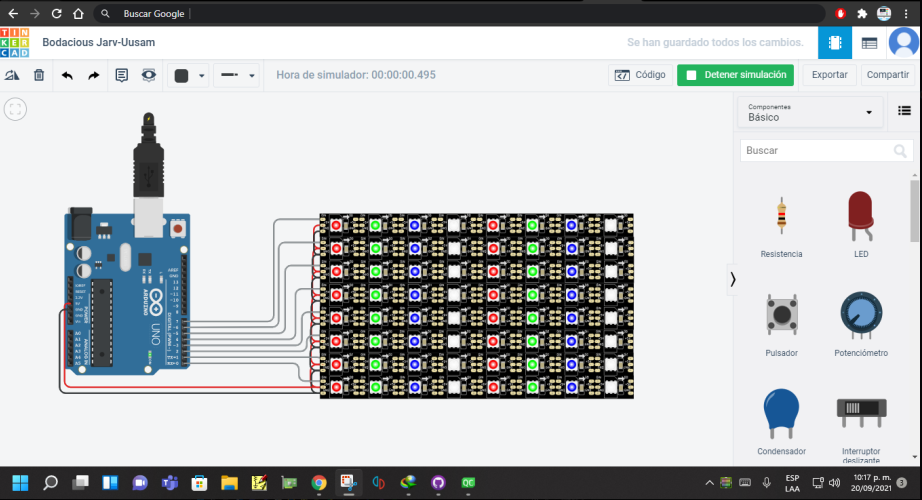
\includegraphics[width=0.5\textwidth]{image1.png}
\end{figure}
\section{dificultades}
he tenido problemas con el tinkercad intentando implementar un arreglo que aun se me dificulta y el repositorio a lo hora de hacerle push y recargar la pagina del repositorio no se modifica lo que he llevado.
\begin{figure}
\centering
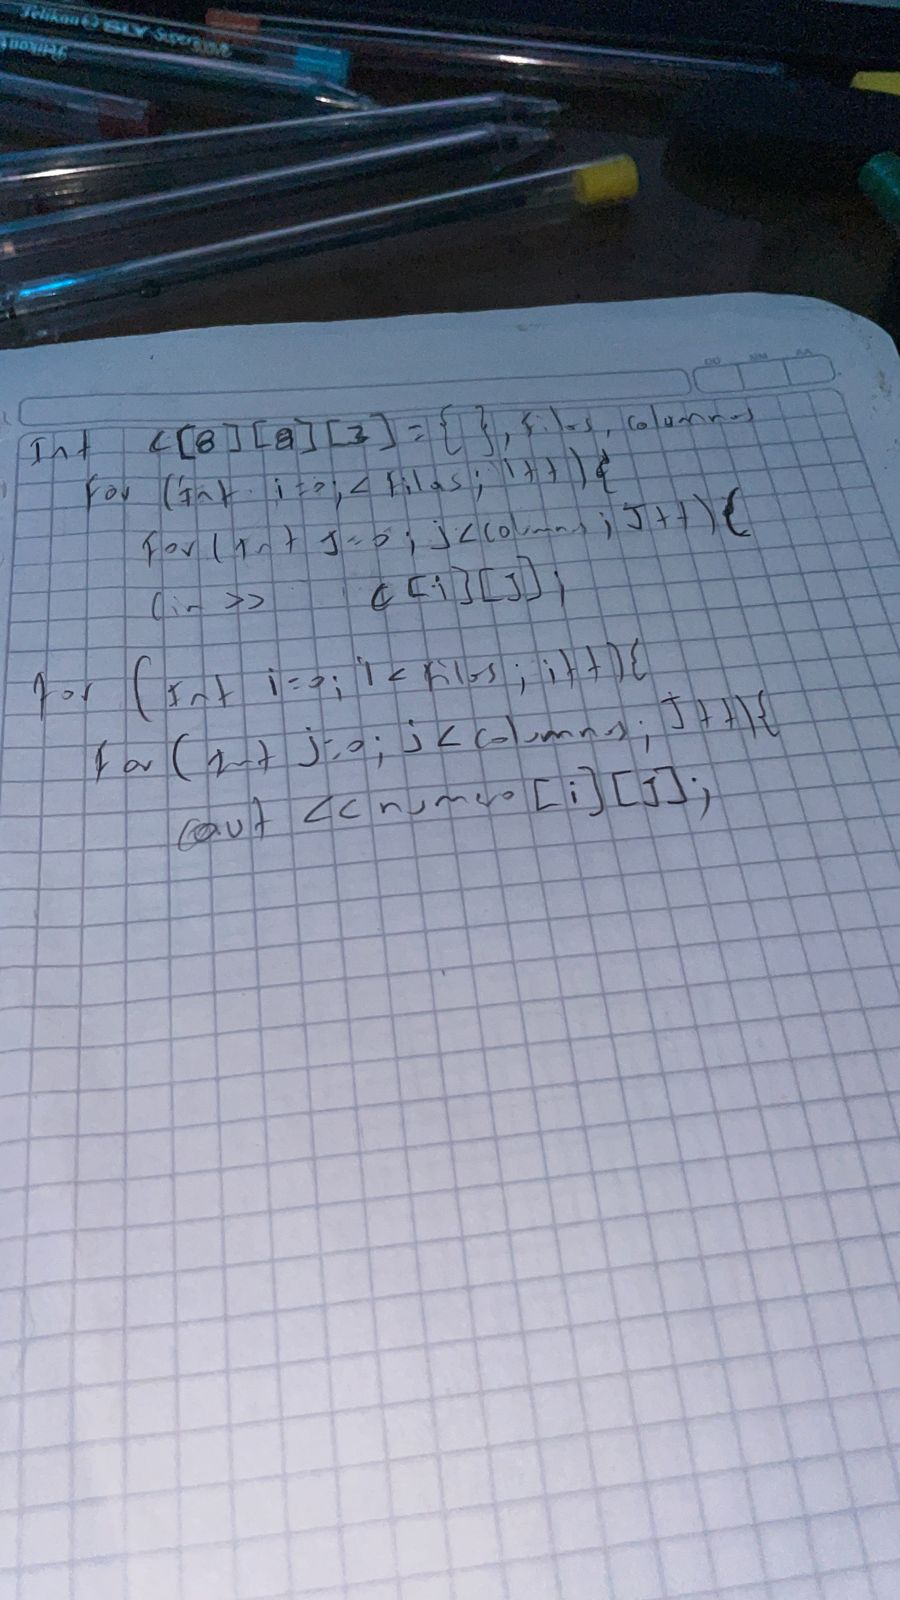
\includegraphics[width=0.5\textwidth]{1.jpeg}
\end{figure}
2.tuvimos un inconveniente con el archivo codificado a la hora de introducirlo al arduino la longitud era muy larga ya que solo tiene 2048 bytes de ram y la maxima cantidad de variables o arreglos a los que pueden llegar es a 500, intentamos dividirlos pero nos dimos cuenta que igual no alcanzaria el espacio y solamente ignoraria esas variables 
longitud inicial:253-2253-2253-282-282-282-2255-2255-2255-2255-2255-2255-2255-2255-2255-2255-2255-2255-2255-2255-2255-2255-2255-2255-271-2194-2253-299-2166-2255-299-2215-2255-2104-2211-2253-2103-2198-2255-298-2200-2249-295-2202-2246-2111-2197-2255-2254-2255-2255-2127-2168-2250-2251-2255-2252-218-219-237-2255-2250-2255-2215-2134-2113-2240-2255-2255-2252-2253-2255-2255-2255-2255-2130-2171-2253-2253-2255-2252-2254-2251-2255-2255-2254-2255-2251-2251-2251-2255-2252-2255-2255-2255-2253-2254-2255-2255-2128-2169-2251-2251-2255-2252-226-243-2112-2242-2253-2249-2117-282-250-2251-2250-2255-2235-2246-2250-2255-2255-2255-2129-2170-2252-2251-2255-2252-2255-2245-2247-2255-2249-2249-2253-2255-2247-2254-2255-2248-2254-2255-2253-2253-2255-2254-2129-2170-2252-2252-2255-2253-239-252-2122-2255-2255-2247-2235-2229-2155-2241-2251-2250-2244-2254-2253-2255-2255-2255-2130-2171-2253-2253-2255-2252-2255-2255-2255-2250-2254-2255-2119-2107-2129-2215-2218-2223-2254-2254-2254-2

longitud a probar:47,28,50,73,15,39,44,21,47,141,39,60,61,25,51,23,19,44,19,19,45,51,25,50,35,21,46,89,34,63,93,32,66,91,34,66,121,34,69,51,28,57,30,25,57,35,15,42,32,22,49,60,26,59,105,29,65,132,56,94,171,57,91,96,40,77,33,25,62,41,22,50,39,24,55,52,27,67,53,30,72,56,33,77,68,41,86,203,66,96,84,26,50,76,28,52,142,60,83,160,64,91,186,81,98,40,8,11,42,14,13,170,75,95,231,46,51,132,49,69,28,15,32,42,22,47,102,30,67,205,59,95,220,68,91,125,38,72,52,20,43,32,15,31,255,255,255,255,255,253,253,253,251,255,254,255,255,254,255,253,253,253,255,254,255,255,255,255,3,3,3,3,3,3,3,3,3,12,3,6,12,3,6,3,3,3,3,3,3,3,3,3
\end{document}